\documentclass[../TG_magistrsko_delo_sections.tex]{subfiles}
\graphicspath{{\subfix{../images/}}}

\begin{document}
V tem poglavju bomo obravnavali topologijo porojemo z linearno ureditvijo. Spoznali bomo družino topoloških prostorov, ki jih imenujemo linearni kontinuum. Gre za neke vrste posplošitev premice realnih števil. Glavni cilj tega poglavja pa bo dokazati, da je linearni kontinuum prostor Šarkovskega.

Naj bo množica $X$ urejena z linearno relacijo $\leq$. Za dana elementa $a, b \in X$, za katera velja neenakost $a<b$, lahko definiramo štiri podmnožice prostora $X$, ki jih imenujemo intervali s krajišči $a$ in $b$. To so:
 %Na množici $X$ imamo dve vrsti odprtih množic, ki ju zapišemo na naslednji način:
\begin{equation*} %\label{eq1}
\begin{split}
(a, b) &= \{x \in X: a< x <b\} \\ 
(a, b] &= \{x \in X: a< x \leq b\} \\ 
[a, b) &= \{x \in X: a \leq x< b\} \\ 
[a, b] &= \{x \in X: a \leq x \leq b\}
\end{split}
\end{equation*}

\begin{opomba}\label{op:intervali}
Interval $(a, b)$ imenujemo odprti interval, intervalu $(a, b]$ rečemo pol odprti interval, interval $[a, b)$ je pol zaprti interval, interval $[a, b]$ pa je zaprti interval.
\end{opomba}

\begin{definicija}
Naj bo $X$ množica z vsaj dvema elementoma urejena z relacijo $\leq$ in naj bo $\mathcal{B}$ družina množic, ki vsebuje intervale naslednjih tipov:
\begin{enumerate}
\item Vsi odprti intervali $(a, b) \in X$. \label{enum:bazna1}
\item Vsi intervali $[a_0, b) \in X$, kjer je $a_0$ najmanjši element (če obstaja) množice $X$. \label{enum:bazna2}
\item Vsi intervali $(a, b_0] \in X$, kjer je $b_0$ največji element (če obstaja) množice $X$. \label{enum:bazna3}
\end{enumerate}
Družina množic $\mathcal{B}$ je baza za topologijo na množici $X$ porojena z ureditvijo $\leq$.
\end{definicija}

\begin{opomba}\label{op:ekstremi}
Če množica $X$ nima najmanjšega elementa, potem baza $\mathcal{B}$ ne vsebuje intervalov tipa~\ref{enum:bazna2} in če množica $X$ nima največjega elementa, potem baza $\mathcal{B}$ ne vsebuje intervalov tipa~\ref{enum:bazna3}.
\end{opomba}

Prepričati se moramo, da zgoraj opisana družina množic $\mathcal{B}$ res predstavlja bazo topologije na množici $X$ urejeni z linearno relacijo $\leq$. Družina podmnožic prostora $X$ je baza topologije na prostoru $X$, če sta izpolnjeni naslednji lastnosti:
\begin{enumerate}[label={(b\arabic*)}]
\item Množice iz družine $\mathcal{B}$ pokrijejo celoten prostor $X$. Torej, vsaka točka $x \in X$ je vsebovana v neki množici $B_1 \in \mathcal{B}$. \label{baza1}
\item Za vsaki množici $B_1, B_2 \in \mathcal{B}$ in vsako točko $x\in B_1 \cap B_2$ obstaja množica $B_3 \in \mathcal{B}$, za katero velja $x \in B_3 \subseteq B_1 \cap B_2$.\label{baza2}
\end{enumerate}

Preverimo najprej pogoj \ref{baza1}.
Najprej moramo preveriti, da je vsaka točka množice $X$ vsebovana v nekem intervalu iz družine $\mathcal{B}$. Če je točka $x$ enaka $a_0$, potem velja $x \in [a_0, a)$ za neko točko $a \in X$. Podobno lahko sklepamo v primeru, ko je $x = b_0$. Če je $x \neq a_0$ in $x \neq b_0$, potem zagotovo obstajata točki $a, b \in X$, za kateri velja $a < x < b$. Tedaj je točka $x$ vsebovana v intervalu $(a, b)$.

Naj bosta $B_1, B_2 \in \mathcal{B}$ poljubni bazni množici z nepraznim presekom in naj bo $x \in B_1 \cap B_2$ poljubna točka iz preseka. Obravnavati moramo več možnosti. 

Recimo, da sta obe množici $B_1, B_2$ tipa~\ref{enum:bazna2}, potem obstajata števili $b_1, b_2 \in X$, za kateri je $B_1 = [a_0, b_1)$ in $B_2 = [a_0, b_2)$. Velja $x \in [a_0, \min\{b_1, b_2\}) \subseteq B_1 \cap B_2$. Podobno lahko sklepamo, ko sta obe množici $B_1, B_2$ tipa~\ref{enum:bazna3}.

Če je ena množica tipa~\ref{enum:bazna2}, ena množica pa tipa~\ref{enum:bazna3}, lahko zapišemo množici z intervali $B_1 = [a_0, b_1)$ in $B_2 = (a_2, b_0]$. Predpostavimo, da je presek teh dveh množic neprazen in da je $x \in B_1 \cap B_2$. Potem je izpolnjena neenakost $a_2 < b_1$, zato velja $x \in (a_2, b_1) \subseteq B_1 \cap B_2$.

Predpostavimo, da je ena množica tipa~\ref{enum:bazna1}, ena množica pa je tipa~\ref{enum:bazna2}. Množici zapišimo s pomočjo intervalov $B_1 = (a_1, b_1), B_1 = [a_0, b_2)$. Denimo, da imata množici $B_1$ in $B_2$ neprazen presek. Potem velja $a_1 < b_2$. Za vsako število $x$ iz preseka $B_1 \cap B_2$ velja $x \in (a_1, \min\{b_1, b_2\}) \subseteq B_1 \cap B_2$. Podoben razmislek deluje tudi v primeru, če je druga množica tipa~\ref{enum:bazna3}.

Na koncu obravnavamo primer, ko sta obe množici tipa~\ref{enum:bazna1}. Zapišimo ju z intervali: $B_1 = (a_1, b_1), B_2 =(a_2, b_2)$. Za vsako število $x \in B_1 \cap B_2$ velja $x \in (\max\{a_1, a_2\}, \min\{b_1, b_2\}) \subseteq B_1 \cap B_2$. Dokazali smo, da družina množic $\mathcal{B}$ res predstavlja bazo topologije na prostoru $X$.

\begin{definicija}
Množici $S$ z vsaj dvema elementoma, ki je urejena z linearno relacijo $\leq$ in opremljena s topologijo, ki jo porodi linearna relacija, pravimo \emph{linearni kontinuum}, če ustreza naslednjima dvema lastnostma:
\begin{enumerate}
\item Vsaka navzgor omejena podmnožica $A \subseteq S$ ima najmanjšo zgornjo mejo v $S$,\label{enum:L1}
\item za vsaki dve števili $x, y \in S$, za kateri velja $x<y$, obstaja število $z \in S$, za katerega je $x<z<y$.\label{enum:L2}
\end{enumerate}
\end{definicija}

Tipičen primer linearnega kontinuuma je množica realnih števil urejena s standardno relacijo $\leq$. Prav tako je vsak interval v realnih številih linearni kantinuum. Poglejmo si še en primer. 

\begin{primer}
Na prostoru $[0, 1] \times [0, 1]$ lahko definiramo linearno relacijo $\preccurlyeq$. Točki $(x, y)$ in $(a, b)$ sta v relaciji $(x, y) \preccurlyeq (a, b)$ natanko tedaj, ko velja $x < a$ ali velja $x = a$ in $y \leq b$. S simboli lahko zapišemo:
$$(x, y) \preccurlyeq (a, b) \Leftrightarrow (x < a) \lor (x = a \land y \leq b).$$
Relacijo $\preccurlyeq$ imenujemo \emph{leksikografska ureditev}. Prostor $[0, 1] \times [0, 1]$ skupaj z leksikografsko ureditvijo je linearni kontinuum. 

\begin{figure}[h]
  \centering
  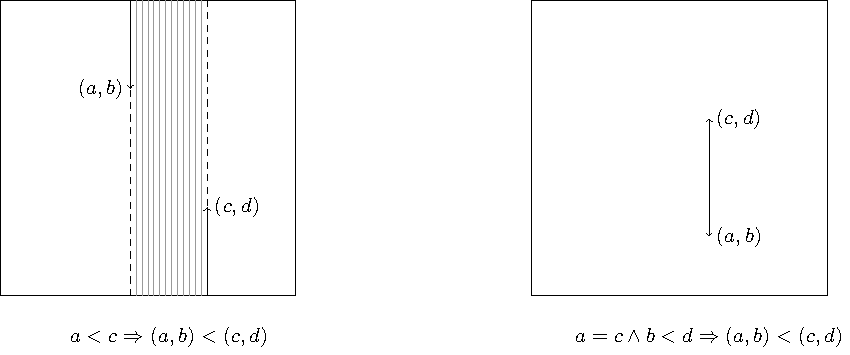
\includegraphics{urejen-kvadrat.pdf}
% \caption[caption za v kazalo]{Dolg caption pod sliko}
  \caption[Primer vektorske slike.]{Relacije pokritja v trditvi~\ref{trd:pokritja} lahko prikažemo z grafom.}
  \label{fig:varsavski_lok}
\end{figure}

Prepričajmo se, da je izpolnjena lastnost~\ref{enum:L1}. Naj bo preslikava $\pi : I \times I \to I$ s predpisom $\pi((x, y)) = x$ pravokotna projekcija na os $x$. Preslikava $\pi$ je zvezna in surjektivna. Naj bo $A$ neprazna in navzgor omejena podmnožica množice $I \times I$. Množica $\pi(A)$ je navzgor omejena podmnožica intervala $I$. Ker ima množica $I$ lastnost~\ref{enum:L1}, obstaja najmanjša zgornja meja $b$ množice $\pi(A)$. Če točka $b$ pripada množici $\pi(A)$, potem množica $b \times I$ seka množico $A$ v neki točki $(b, c)$. Ker je množica $b \times I$ ekvivalentna množici $I$, ima lastnost~\ref{enum:L1}, zato obstaja najmanjša zgornja meja $(b, c')$ za množico $(b \times I) \cap A$. Ta točka je tudi najmanjša zgornja meja množice $A$.
V primeru, ko točka $b$ ne leži v množici $\pi(A)$, je najmanjša zgornja meja množice $A$ točka $(b, 0)$. Res, če je za neki števili $d < b$ in $e \in I$ točka $(d, e)$ najmanjša zgornja meja množice $A$, potem je $d$ manjša zgornja meja množice $\pi(A)$ kot $b$, kar je protislovje s tem, da je $b$ najmanjša zgornja meja množice $\pi(A)$.
Prostor $I \times I$ ima tudi lastnost~\ref{enum:L2}. Naj bosta $(x, y)$ in $(a, b)$ dve točki v prostoru $I \times I$, ki ustrezata relaciji $(x, y) \preccurlyeq (a, b)$. Če je $x < a$, potem obstaja število $u$, za katerega velja $x<u<a$. Sedaj lahko zapišemo relacijo $(x, y) \preccurlyeq (u, 0) \preccurlyeq (a, b)$. V primeru, ko je $x=a$ in $y<b$, obstaja število $v$, ki izpolnjuje pogoj $y<v<b$. Sedaj je izpolnjena relacija $(x, y) \preccurlyeq (x, v) \preccurlyeq (a, b)$. 
\end{primer}



\begin{trditev}
Linearno urejena množica $X$ s topologijo porojeno z linearno relacijo $\leq$ je linearni kontinuum natanko tedaj, ko je povezana.
\end{trditev}
\begin{proof}
Predpostavimo, da je prostor $X$ opremljen s topologijo porojeno z linearno relacijo $\leq$. Denimo, da $X$ ni linearni kontinuum. Potem ne zadošča pogoju~\ref{enum:L1} ali ne zadošča pogoju~\ref{enum:L2}. Recimo, da ne množica $X$ ne zadošča pogoju~\ref{enum:L1}. Naj bo $A$ neprazna podmnožica množice $X$, ki je navzgor omejena s točko $b$, vendar nima najmanjše zgornje meje. Naj bo $U$ množica vseh zgornjih mej množice $A$. Če točka $x$ leži v množici $U$, potem točka $x$ ni najmanjša zgornja meja množice $A$, zato obstaja $z \in X$, za katerega je $z < x$ in $z$ je tudi zgornja meja množice $A$. Množica $\{y \in X; y > z\}$ je odprta neprazna, saj vsebuje točko $x$. Vsak njen element je večji os točke $z$ in je tako zgornja meja množice $A$. Torej, množica $\{y \in X; y > z\}$ je odprta podmnožica množice $U$, ki vsebuje točko $x$. Ugotovili smo, da je množica U odprta podmnožica prostora $X$. Množica $U$ je neprazna, saj vsebuje točko $b$. 

Naj bo $w$ poljubna točka iz množice $X \setminus U$. Potem $w$ zagotovo ni zgornja meja množice $A$, zato obstaja točka $a \in A$, za katero je $w < a$. Množica $\{y \in X; y< a\}$ je odprta in ne vsebuje nobene zgornje meje množice $A$, zato je vsebovana v množici $X \setminus U$. Sklepamo, množica $X \setminus U$ vsebuje odprto okolico točke $w$ in je zato odprta množica. 

Ker sta množici $U$ in $X \setminus U$ obe neprazni in odprti, tvorita separacijo prostora $X$. 

Recimo, da prostor $X$ ne ustreza pogoju~\ref{enum:L2}. To pomeni, da odbstajata elementa $a$ in $b$ , prostoru $X$, za katari velja $a < b$, vandar ne obstaja točka $c \in X$, za katero je izpolnjena neenakost $a < c < b$. Definiramo množici $U := \{x \in X, x <b\}$ in $V:= \{x\in X;x>a\}$. Ker med točko $a$ in točko $b$ ne leži nobena točka iz $X$, sta množici $U$ in $V$ disjunktni. Ker je relacija $<$ relacija linearne urejenost, za vsaki točki $x$ in $y$ velja $x < y$ ali $y < x$. Za poljubno točko $x \in X$ lahko velja $x<a$, $a<x$ ali $x=a$.
Če je $x<a$, zaradi tranzitivnosti sklepamo, da je $x<b$, kar pomeni, da je točka $x$ vsebovana v množici $U$. Če je $x=a$, velja $x=a<b$, zato točka $x$ pripada množici $U$. Kadar je $a<x$, točka $x$ pripada množici $V$. Prepričali smo se, da je $U \cup V = X$. Množici $U$ in $V$ sta neprazni, saj prva vsebuje točko $a$, druga pa vsebuje točko $b$. Množici sta tudi odprti in tvorita particijo množice $X$. Prepričali smo se, da je množica $X$ nepovezana.
Torej, če je prostor $X$ povezan, je linearni kontinuum.

Predpostavimo, da je $X$ nepovezana množica z lastnostjo~\ref{enum:L1}. Naj bosta množici $U$ in $V$ neprazni odprti množici, ki tvorita particijo prostora $X$. Naj bo $a$ točka iz množice $V$ in naj obstaja taka točka $b \in U$, ki ustreza relaciji $b<a$. Če taka točka ne obstaja, zamenjamo imeni za množici $U$ in $V$. Množica $Z = \{x \in U, x<a\}$ je odprta množica, saj jo dobimo kot presek odprte množice $U$ in odprte množice $\{x \in X, x<a\}$. Množica $Z$ je neprazna, saj vsebuje točko $b$. Ker je množica $Z$ navzgor omejena, ima najmanjšo zgornjo mejo $z$.

Predpostavimo, da je točka $z$ vsebovana v množici $U$. Množica $U$ je odprta, zato obstaja interval v $U$, ki vsebuje točko $z$. Interval ne more vsebovati točke $a$, zato mora biti oblike $\{x \in X, x<j\}$ ali $\{x \in X, k<x<j\}$ za neko število $j$ in morda $k$. V obeh primerih velja $z<j<a$. Naj bo $W:=\{x \in X, z<x<j\}$ množica vseh točk iz $X$, ki ležijo med točkama $z$ in $j$. Če je $x \in W$, potem je $x$ iz množice $U$ in velja $x<a$, kar pomeni, da je $x$ element množice $Z$. To je v protislovju s predpostavko, da je $z$ zgornja meja množice $Z$. Množica $W$ je prazna množica, zato med točkama $j$ in $z$ ne leži nobena točka iz $X$. Množica $X$ ne izpolnjuje pogoja~\ref{enum:L2} in zato ni linearni kontinuum.
\end{proof}

Trditev, da je linearni kontinuum prostor Šarkovskega, bomo dokazali tako, da bomo sledili dokazu, ki smo ga zapisali za realna števila in izreke, leme, trditve in definicije iz dokaza za realna števila prilagodili linearnemu kontinuumu. Najprej bomo obravnavali posplošitve v poglavju~\ref{sec:intervali}. Zapišimo in dokažimo posplošitev izreka o vmesni vrednosti za linearni kontinuum.

\begin{izrek}[izrek o vmesni vrednosti za linearni kontinuum]
Naj bo $f : X \to Y$ zvezna funkcija, kjer je $X$ povezan prostor in $Y$ urejen prostor s topologijo urejenih množic. Če sta $a$ in $b$ dve točki v prostoru $X$ in je $r$ točka v prostoru $Y$, ki leži med točkama $f(a)$ in $f(b)$, potem obstaja točka $c \in X$, za katero velja $f(c) = r$.
\end{izrek}
\begin{proof}
Privzemimo predpostavke izreka. Množici $=f(X) \cap (-\infty, r)$ in $B=f(X) \cap (r, \infty)$ sta disjunktni in neprazni, saj ena množica vsebuje točko $f(a)$, druga pa točko $f(b)$. Obe sta odprti v $f(X)$ saj smo ju dobili kot presek odprtega intervala z množico $f(X)$. Če ne obstaja taka točke $c \in X$, da je $f(c) = r$, potem je $f(X)$ unija množic $A$ in $\mathcal{B}$. Na ta način smo dobili separacijo množice $f(X)$, kar pa je protislovje, saj je slika povezane množice z zvezno preslikavo povezana.
\end{proof}

Sedaj dokažimo posplošitev leme~\ref{lem:dovetail}

\begin{lema}\label{lem:K}
Naj bo $L$ linearni kontinuum s topologijo urejenih množic. Naj bosta $I$ in $J$ zaprta intervala v $L$ in $f:L \to L$ zvezna funkcija. Če je $J \subseteq f(I)$, obstaja zaprt interval $K \subseteq I$, za katerega je $f(K) = J$.
\end{lema}
\begin{proof}
Izberemo taki točki $p, q \in I$, da velja $p<q$ in $J=[f(p), f(q)]$ ali $J=[f(q), f(p)]$. Definiramo točko $r \in [p, q)$:
$$r:= \sup\{x \in [p, q] : f(x) = f(p)\}.$$
Trdimo, da je $f(r) = f(p)$. V nasprotnem primeru obstaja odprta množica $V$, ki vsebuje točko $f(r)$ in ne vsebuje točke $f(p)$. To je res, ker je prostor $L$ Hausdorffov. Zaradi zveznosti funkcije $f$ obstaja taka odprta okolica $U$ točke $r$, da je $f(U) \subseteq V$. Ker je $L$ linearni kontinuum obstaja taka točka $p \leq r' < r$, za katero je interval $[r', r]$ vsebovan v množici $U$. Torej je $f([r', r]) \subseteq V$, kar pomeni, da $f(p) \notin f([r', r])$. To pa je protislovje z definicijo točke $r$ kot supremum množice.
Sedaj definiramo točko $s \in (r, q]$:
$$s:= \inf\{x \in [r, q] : f(x) = f(q)\}.$$ 
Enako kot prej se prepričamo, da je $f(s) = f(q)$. Zapišimo $Q = [r, s]$ in pokažimo, da je $f(Q) = J$. Izrek o vmesni vrednosti zagotavlja, da je interval $J$ vsebovan v množici $f([r, s])$. Velja tudi $f([r, s]) \subseteq J$, saj v nasprotnem primeru obstaja $r<x<s$, za katerega velja $f(x) \notin J$. Če je $f(x) < f(p) < f(q)$ ali $f(q) < f(p) < f(x)$, potem po izreku o vmesni vrednosti obstaja tak $x'$, da velja $r<x<x'<s$ in $f(p) = f(x')$. to pa je protislovje z definicijo točke $r$ kot supremum. Če je $f(x) < f(q) < f(p)$ ali $f(p) < f(q) < f(x)$, to privede do protislovja z definicijo točke $s$ kot infimum. To pomeni, da res velja $J = f(Q)$.
\end{proof}

Tudi lemo~\ref{lem:zanka1} moramo prilagoditi za linearni kontinuum.

\begin{lema}
Naj bo $L$ linearni kontinuum v topologiji urejenih množic. Naj bosta $I$ zaprt interval v $L$ in $f:L \to L$ zvezna funkcija. Če je $I \subseteq f(I)$, potem ima $f$ negibno točko $x \in I$.
\end{lema}
\begin{proof}
S pomočjo leme~\ref{lem:K} ugotovimo, da obstaja zaprt interval $Q \subseteq I$, za katerega je $f(Q) = I$. Pokazali bomo, da ima funkcija $f$ negibno točko v intervalu $Q$. Predpostavimo, da funkcija $f$ na intervalu $Q$ nima negibne točke. Potem lahko zapišemo $Q = A \cup B$, kjer je:
\begin{equation*} %\label{eq1}
\begin{split}
A &= \{x \in L : x < f(x)\}, \\ 
B &= \{x \in L : x > f(x)\}.
\end{split}
\end{equation*}
Trdimo, da je množica $A$ odprta. Za vsako točko $x \in A$ lahko izberemo točko $z \in (x, f(x))$ in odprto okolico $U \subseteq  (-\infty, z)$ točke $x$, za katero velja $f(U) \subseteq (z, \infty)$. Ker je množica $U$ podmnožica množoce $A$, je točka $x$ notranja točka množice $A$. Množica $A$ je odprta. Podobno lahko dokažemo, da je množica $\mathcal{B}$ odprta. Množici $Q \cap A$ in $Q \cap B$ sta odprti podmnožici množice $Q$ za kateri velja $Q = (Q \cap A) \cup (Q \cap B)$. Radi bi videli, da sta množici $Q \cap A$ in $Q \cap B$ neprazni. Zapišimo $I = [c, d]$. Ker je $f(Q) = I$, obstaja $x' \in Q$, za katerega je $f(x') =d$. Ker $f$ nima fiksne točke na $Q$, je $x' \neq d$. Interval $Q$ je pomnožica intervala $I$, zato velja $x' < f(x') = d$, kar pomeni, da je $x' \in Q \cap A$. Analogno poiščemo točko $x'' \in Q - \{c\}$ z lastnostjo: $f(x'') = c$ in $x'' \in Q \cap B$. Torej, množici $Q \cap A$ in $Q \cap B$ tvorita separacijo povezanega prostora $Q$, kar je protislovje. Funkcija $f$ ima negibno točko v intervalu $Q$.
\end{proof}

Preostanek poglavja velja tudi za intervale v linearnem kontinuumu.

V poglavju~\ref{stefan_zap} moramo razložiti besedišče, da je primerno za linearni kontinuum. Naj bo $L$ linearni kontinuum s topologijo, ki jo poraja linearna relacija $\leq$. Za točki $x$ in $y$ iz linearnega kontinuuma $L$ rečemo, da $x$ leži levo od $y$ natanko tedaj, ko velja $x<y$. Ekvivalentno rečemo, da $x$ leži desno od $y$, če velja $y<x$. Ker je $L$ linearni kontinuum, za vsaki točki $x, y \in L$ obstaja točka $z$, ki izpolnjuje pogoj $x<z<y$. Tako lahko za center cikla $\mathcal{O}$ v linearnem kontinuumu izberemo poljubno točko $c \in L$, ki izpolnjuje pogoj $p< c <q$. Pri definiciji~\ref{def:stef-zap},kjer smo definirali Štefanovo zaporedje moramo pojasniti točko~\ref{eq:š3}. Kaj pomeni, da sta zaporedji 
$\left \{ x_{2j} \right \}_{j=0}^{\left \lfloor \frac{n}{2} \right \rfloor}$ 
    in
$\left \{ x_{2j+1} \right \}_{j=0}^{\left \lfloor \frac{n}{2} \right \rfloor}$
 strogo monotoni in se oddaljujeta od točke $c$?
Povedati želimo, da vsak naslednji člen zaporedja, ki leži levo od točke $c$, leži levo od prejšnjega člena. Vsak naslednji člen zaporedja, ki leži desno od točke $c$ pa leži desno od prejšnjega člena. Preostanek poglavja~\ref{stefan_zap} in poglavji~\ref{konssz} in~\ref{sec:dokaz-izreka} veljajo tudi za funkcije in intervale definirane na linearnem kontinuumu, zato je linearni kontinuum tudi prostor Šarkovskega.


\end{document}